\documentclass{jsarticle}
\usepackage[dvipdfmx]{hyperref}
\usepackage[dvipdfmx]{graphicx}
\usepackage{amssymb,amsmath,amsthm}
\usepackage{listings,jlisting}
\usepackage{newtxtt}
\usepackage{cases}
\usepackage{here}
\usepackage[utf8]{inputenc}
\lstset{
  language=Python,      
  basicstyle={\small},%
  identifierstyle={\small},%
  commentstyle={\small\itshape},%
  keywordstyle={\small\bfseries},%
  ndkeywordstyle={\small},%
  stringstyle={\small\ttfamily},
  frame={tblr},
  breaklines=true,
  columns=[l]{fullflexible},%
% numbers=left,%
  xrightmargin=0zw,%
  xleftmargin=3zw,%
  numberstyle={\scriptsize},%
  stepnumber=1,
  numbersep=1zw,%
  lineskip=-0.5ex%
}
\date{\today}
\author{山田龍}
\title{}
\begin{document}
\maketitle
\section{常微分方程式}
\subsection{課題1}
\begin{equation}
    \frac{dx}{dt} = \frac{x + \sqrt{x^2 + t^2}}{t}
\end{equation}\label{eq:1}
\eqref{eq:1}の形の常微分方程式を解くことを考える。
$t_0=1,x_0 = 0$を初期条件としてルンゲクッタ公式を用いて$t=1$まで計算する。

\begin{figure}[htbp]
    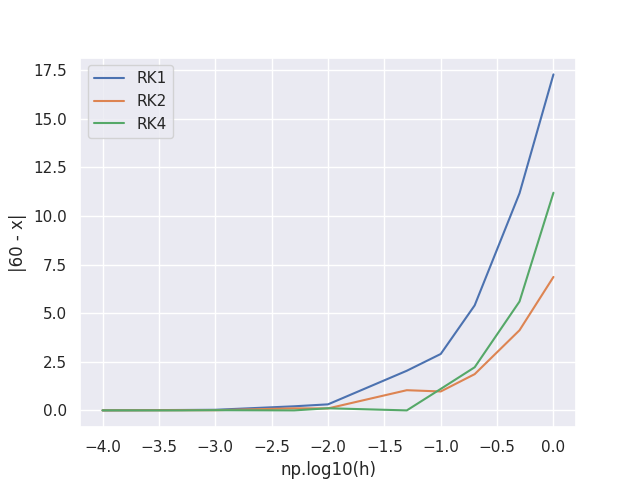
\includegraphics[clip,width=10.0cm]{./runge_kutta_error.png}
    \caption{RungeKutta法の誤差}
    \label{fig:1}
\end{figure}
1次、2次、4次のルンゲクッタ法を用いて時間刻み幅$h$を変化させた結果が図\ref{fig:1}のようになる。
横軸が刻み幅の対数、縦軸が$t=1$での真値からのズレ$|60 - x|$の対数である。対数の基底は$10$にとった。
どの刻み幅においても、次数の高いルンゲクッタ法が誤差が少なかった。
またプロットの傾きがどれも1程度であるから、$error \propto h$であることがわかる。

4次のルンゲクッタ法においてメモリを節約する工夫がある。
ソースコード\ref{code:1}が一般的なルンゲクッタ法の実装である。
$dh$を刻み幅として、$x$を更新している。
これをソースコード\ref{code:2}のようにすると、$k1,k2,k3,k4$の代わりに、$x$のコピー、$k$の2つで計算できるようになるので改善している。
\begin{lstlisting}[caption=通常の4次のルンゲクッタ,label={code:1}]
    while t < t_end:
        k_one = dh * f(x, t)
        k_two = dh * f(x + k_one / 2, t + dh / 2)
        k_three = dh * f(x + k_two / 2, t + dh / 2)
        k_four = dh * f(x + k_three, t + dh)
        x = x + k_one / 6 + k_two / 3 + k_three / 3 + k_four / 6
        t += dh

\end{lstlisting}
\begin{lstlisting}[caption=メモリを節約する4次のルンゲクッタ,label={code:2}]
    while t < t_end:
        x_cur = x
        k = dh * f(x, t)
        x += k / 6
        k = dh * f(x_cur + k / 2, t + dh / 2)
        x += k / 3
        k = dh * f(x_cur + k / 2, t + dh / 2)
        x += k / 3
        k = dh * f(x_cur + k, t + dh)
        x += k / 6
        t += dh

\end{lstlisting}

\subsection{課題2}
ケプラー運動をルンゲクッタ法を用いて解くことを考える。
中心にある動かない質点の周りを回る質点の運動を考える。
計算にルンゲクッタ法を用いると、シンプレクティックな計算法ではない、
つまりステップの更新による座標変換が正準変換になっていないので
エネルギーは保存しないことを確認する。
設定は
\begin{align}
    \frac{dx}{dt} = u\\
    \frac{dy}{dt} = v\\
    \frac{du}{dt} = - \frac{x}{(x^2 + y^2)^{3/2}} = f(x, y)\label{eq:u}\\
    \frac{dv}{dt} = - \frac{y}{(x^2 + y^2)^{3/2}}=g(x,y)\label{eq:v}\\
\end{align}
速度の微分に関する式\eqref{eq:u}、\eqref{eq:v}は中心力を意味する。
初期条件は$x(0) = 3,y(0)=0,u(0)=0.3,v(0)=2$ととる。
また、系の全エネルギーは
\begin{equation}
    E = \frac{1}{2} (u^2 + v^2) - \frac{1}{\sqrt{x^2 + y^2}}
\end{equation}
刻み幅を$h$として、時間発展の計算方法は以下のようになる。
\begin{align}
    k_{1x} &= h  \times u)\\
    k_{1y} &= h  \times v\\
    k_{1u} &= h  \times f(x, y)\\
    k_{1v} &= h  \times g(x, y)\\
    k_{2x} &= h  \times (u + k_{1u})\\
    k_{2y} &= h  \times (v + k_{1v})\\
    k_{2u} &= h  \times f(x + \frac{k_{1x}}{2}, y+ \frac{k_{1y}}{2})\\
    k_{2v} &= h  \times g(x + \frac{k_{1x}}{2}, y+ \frac{k_{1y}}{2})\\
    k_{3x} &= h  \times (u + k_{2u})\\
    k_{3y} &= h  \times (v + k_{2v})\\
    k_{3u} &= h  \times f(x + \frac{k_{2x}}{2}, y+ \frac{k_{2y}}{2})\\
    k_{3v} &= h  \times g(x + \frac{k_{2x}}{2}, y+ \frac{k_{2y}}{2})\\
    k_{4x} &= h  \times (u + k_{3u})\\
    k_{4y} &= h  \times (v + k_{3v})\\
    k_{4u} &= h  \times f(x + k_{3x}, y+ k_{1y})\\
    k_{4v} &= h  \times g(x + k_{3x}, y+ k_{1y})\\
    \tilde{x} &= x + \frac{k_{1x} + 2k_{2x} + 2k_{3x} + k_{4x}}{6}
\end{align}
$y,u,v$も同様に更新する。
空間座標を表示すると図\ref{fig:kepler}のようになる。
原点を中心に楕円を描いている。
\begin{figure}[htbp]
    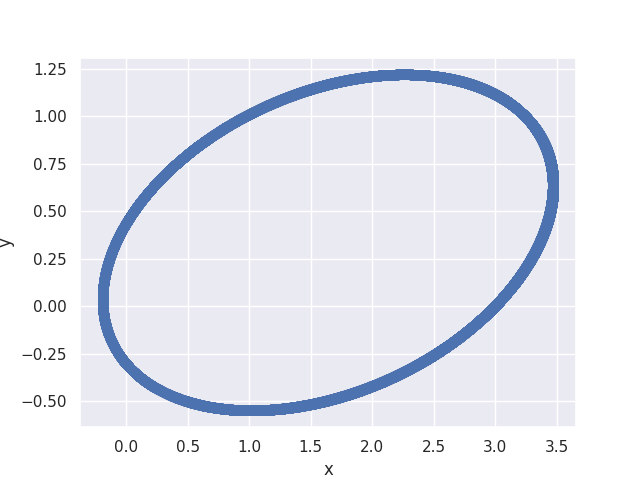
\includegraphics[clip,width=10.0cm]{./kepler.png}
    \caption{kepler運動}
    \label{fig:kepler}
\end{figure}
エネルギーの変化は図\ref{fig:2}のようになる。刻み幅を小さくするほどエネルギーの損失は少なくなる。
\begin{figure}[htbp]
    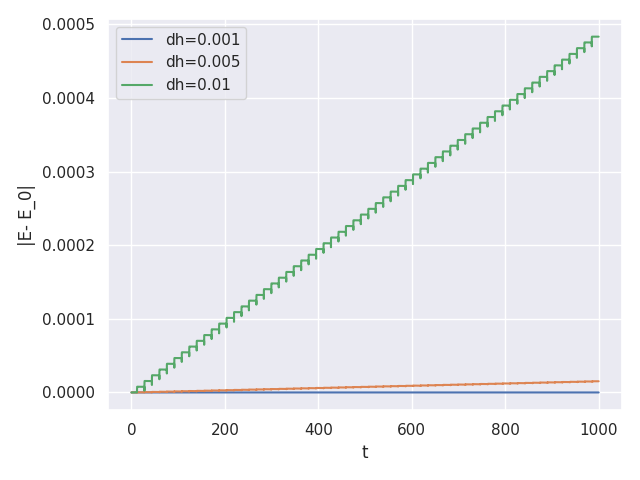
\includegraphics[clip,width=10.0cm]{./energy.png}
    \caption{エネルギーの変化}
    \label{fig:2}
\end{figure}
また、大きな刻み幅についても計算し両軸に対数を取って表示した結果は図\ref{fig:3}のようになる。
$0.01$の刻み幅を境にエネルギー誤差が大きくなりシミュレーションできていないことがわかる。
%todo:1なぜ?
\begin{figure}[htbp]
    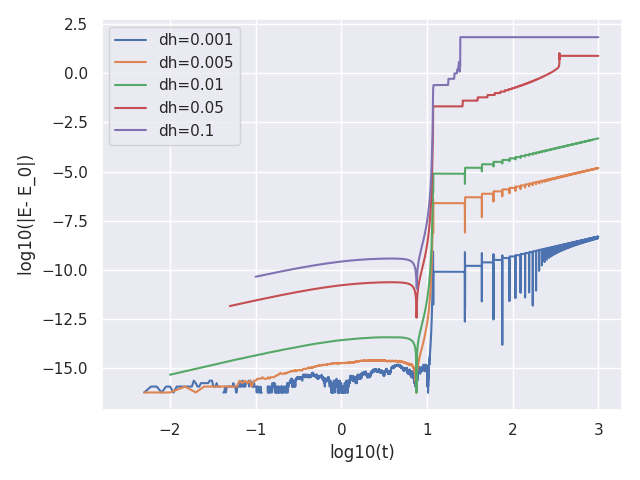
\includegraphics[clip,width=10.0cm]{./energy_log.png}
    \caption{log(エネルギーの変化)}
    \label{fig:3}
\end{figure}

\section{偏微分方程式の境界問題}
\subsection{課題1}
二次元ラプラス方程式
\begin{equation}
    \frac{\partial^2u}{\partial x^2} +     \frac{\partial^2u}{\partial y^2} = 0
\end{equation}
を解くことを考える。一般に、境界での法線微分係数を与える(Neumann b.c.)か直接境界値を与える(Dirichlet b.c.)と内部の解は一意に定まる。
ここではDirichlet b.c.の下で考える。
二階微分は5点差分公式を使うと
\begin{equation}
    f''(x_i) = \frac{-f_{i-2}+16f_{i-1}-30f_{i}+16f_{i+1}-f_{i+2}}{12h^2} + O(h^4)
\end{equation}
と差分化されるので、インデックスi,jで指定される二次元空間の各点において方程式を一つ得る。
境界の値は与えられているので空間のグリッドを$n\times n$に切ると、
$n-1 \times n-1$個の未知数、つまり各点での$u$、を求めるための$n-1 \times n-1$個の方程式を得る。
したがって、この問題は連立方程式の解に帰着できる。
この方法によって、以前作成したSOR法を用いてといた結果が図\ref{fig:5}のようになる。
%todo:厳密界との比較
\begin{figure}[htbp]
    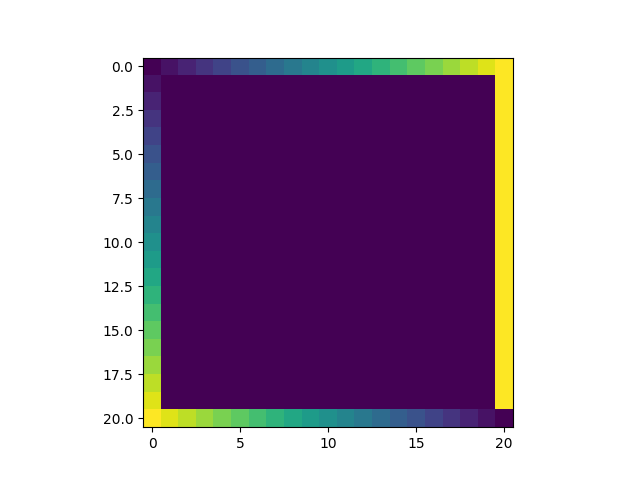
\includegraphics[clip,width=8.0cm]{./init.png}
    \caption{初期条件のみ表示した図}
    \label{fig:4}
\end{figure}
\begin{figure}[H]
    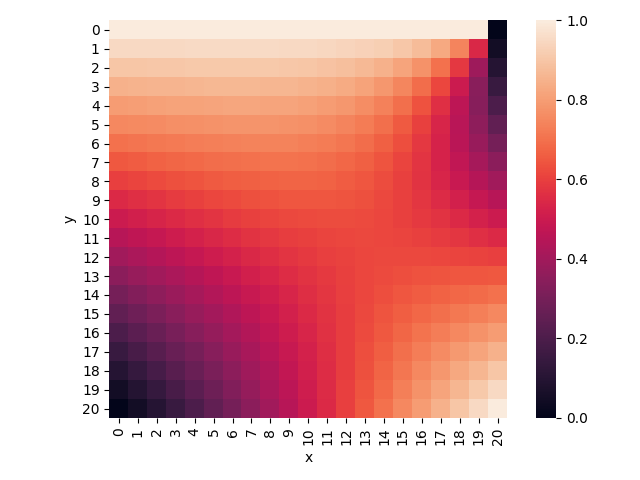
\includegraphics[clip,width=8.0cm]{./pde.png}
    \caption{ラプラス方程式の解、y軸の目盛りは無視すること。原点は左下}
    \label{fig:5}
\end{figure}

\section{移流方程式}
\subsection{課題1}
移流方程式
\begin{equation}
    \frac{\partial u}{\partial t} + c\frac{\partial u}{\partial x} = 0
\end{equation}
を境界条件
\begin{equation}
    u(x+1, t) = u(x, t)
\end{equation}
と初期条件
\begin{equation}
    u(x, 0) = \sin^{100} (\pi x) 
\end{equation}
の下で解くことを考える。
例えば中心差分法で差分化すれば、上付き添字を時刻、下付き添字を座標に関するインデックスとおいて、
\begin{align}
    \frac{u^{n+1}_j - u^{n}_j}{\Delta t} = c \frac{u^n_{j+1} - u^n_{j-1}}{2\Delta x}
\end{align}
と書ける。したがって、
\begin{align}
    u^{n+1}_j  =  u^{n}_j+ c \Delta t\frac{u^n_{j+1} - u^n_{j-1}}{2\Delta x}
\end{align}
と更新される。中心差分法をこのまま使うと、図\ref{fig:6}のように安定ではない。
しかし、4段4位の古典ルンゲクッタ法を使えば安定に計算できて結果が、図\ref{fig:7}のようになる。
風上差分法を用いれば、クーラン条件を満たしている限り計算は安定であり、図\ref{fig:8}のようになる。
クーラン条件はフォン・ノイマンの安定性解析において更新される関数を
フーリエ級数として表し、すべての波数においてスケールが発散しないことを要請した結果として現れる。
風下差分法を使うと、計算が不安定になって壊れいる様子も得られた(図\ref{fig:9})。
\begin{figure}[htbp]
    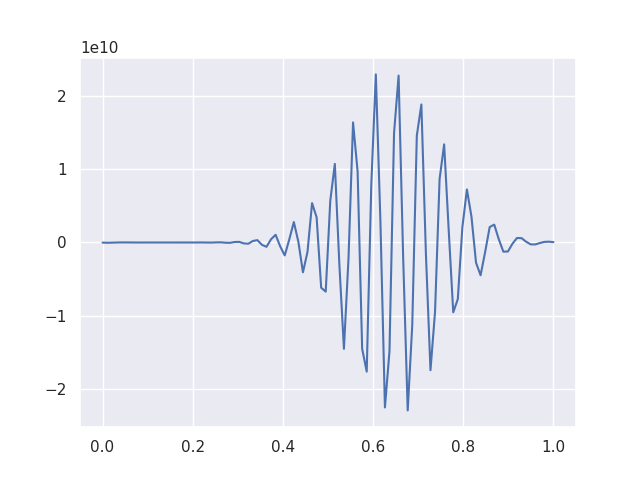
\includegraphics[clip,width=10.0cm]{./adv_center.png}
    \caption{中心差分法,t=1での様子}
    \label{fig:6}
\end{figure}

\begin{figure}[H]
    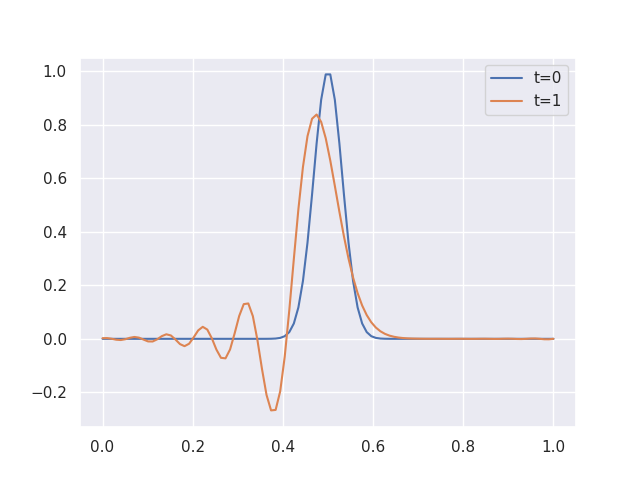
\includegraphics[clip,width=10.0cm]{./adv_center_rk.png}
    \caption{中心差分法RK}
    \label{fig:7}
\end{figure}

\begin{figure}[H]
    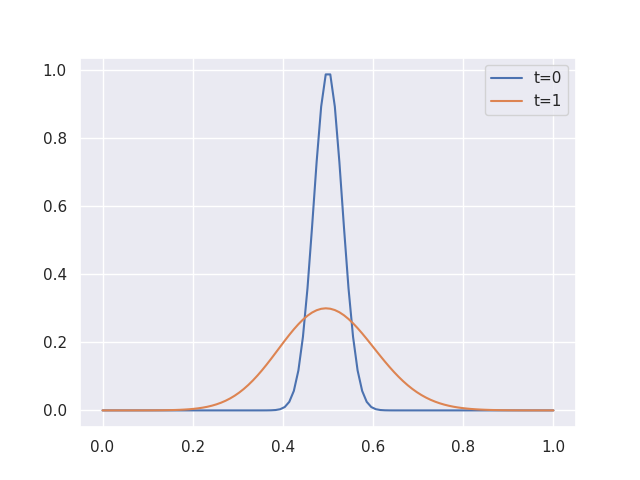
\includegraphics[clip,width=10.0cm]{./adv_upwind_rk.png}
    \caption{風上差分法}
    \label{fig:8}
\end{figure}

\begin{figure}[H]
    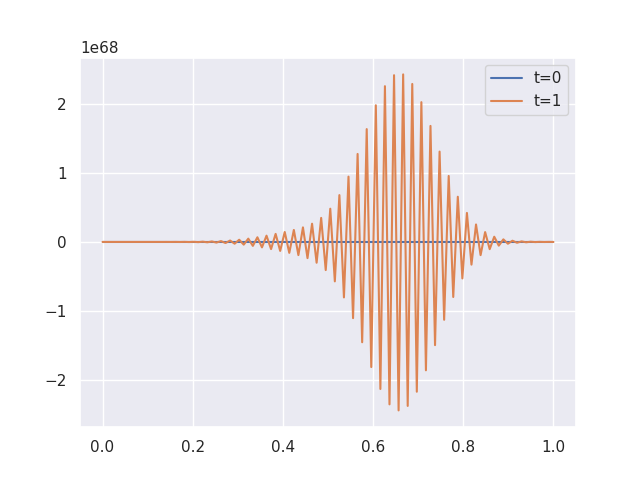
\includegraphics[clip,width=10.0cm]{./adv_downwind_rk.png}
    \caption{風下差分法}
    \label{fig:9}
\end{figure}
\section{ソースコード}
\subsection{常微分方程式}
\subsubsection{課題1}
\begin{lstlisting}[caption=Runge-Kutta法,label=参照ラベル]
import numpy as np
import matplotlib.pyplot as plt
import seaborn as sns


def f(x, t):
    res = x + np.sqrt(x ** 2 + t ** 2)
    res = res / t
    return res


def runge_kutta_one(x, dh, t, t_end):
    while t < t_end:
        x = x + dh * f(x, t)
        t += dh
    return x


def runge_kutta_two(x, dh, t, t_end):
    while t < t_end:
        k_one = dh * f(x, t)
        # Heun法を採用
        k_two = dh * f(x + k_one / 2, t + dh / 2)
        x = x + k_one / 2 + k_two / 2
        t += dh
    return x


def runge_kutta_four(x, dh, t, t_end):
    while t < t_end:
        k_one = dh * f(x, t)
        k_two = dh * f(x + k_one / 2, t + dh / 2)
        k_three = dh * f(x + k_two / 2, t + dh / 2)
        k_four = dh * f(x + k_three, t + dh)
        x = x + k_one / 6 + k_two / 3 + k_three / 3 + k_four / 6
        t += dh
    return x


def runge_kutta_four_efficient(x, dh, t, t_end):
    while t < t_end:
        x_cur = x
        k = dh * f(x, t)
        x += k / 6
        k = dh * f(x_cur + k / 2, t + dh / 2)
        x += k / 3
        k = dh * f(x_cur + k / 2, t + dh / 2)
        x += k / 3
        k = dh * f(x_cur + k, t + dh)
        x += k / 6
        t += dh
    return x


def plot_runge_kutta():
    sns.set_theme()
    x, t = 0, 1
    tend = 11
    one_ls = []
    two_ls = []
    four_ls = []
    ans = 60
    dh_ls = [
        0.0001,
        0.0003,
        0.0007,
        0.001,
        0.003,
        0.007,
        0.01,
        0.03,
        0.07,
        0.1,
        0.2,
        0.5,
        1,
    ]
    for dh in dh_ls:
        one_ls.append(np.fabs(ans - runge_kutta_one(x, dh, t, tend)))
        two_ls.append(np.fabs(ans - runge_kutta_two(x, dh, t, tend)))
        four_ls.append(np.fabs(ans - runge_kutta_four_efficient(x, dh, t, tend)))
    log_dh = np.log10(dh_ls)
    plt.plot(log_dh, np.log10(one_ls), label="RK1")
    plt.plot(log_dh, np.log10(two_ls), label="RK2")
    plt.plot(log_dh, np.log10(four_ls), label="RK4")
    plt.xlabel("log10(h)")
    plt.ylabel("log10(|60 - x|)")
    plt.legend()
    plt.savefig("runge_kutta_error.png")


if __name__ == "__main__":
    plot_runge_kutta()
\end{lstlisting}
\subsubsection{課題2}
\begin{lstlisting}[caption=エネルギー誤差の計算,label=参照ラベル]
import numpy as np
import matplotlib.pyplot as plt
import seaborn as sns


def sum_square(vector):
    return vector[0] ** 2 + vector[1] ** 2


def duv(position):
    denominator = sum_square(position) ** 1.5
    return np.array([-position[0] / denominator, -position[1] / denominator])


def dxy(velocity):
    return velocity


def runge_kutta_one(position, velocity, dh):
    k_one_pos = dh * dxy(velocity)
    k_one_vel = dh * duv(position)
    position += k_one_pos
    velocity += k_one_vel
    return position, velocity


def runge_kutta_four(position, velocity, dh):
    k_one_pos = dh * dxy(velocity)
    k_one_vel = dh * duv(position)
    k_two_pos = dh * dxy(velocity + k_one_vel / 2)
    k_two_vel = dh * duv(position + k_one_pos / 2)
    k_three_pos = dh * dxy(velocity + k_two_vel / 2)
    k_three_vel = dh * duv(position + k_two_pos / 2)
    k_four_pos = dh * dxy(velocity + k_three_vel)
    k_four_vel = dh * duv(position + k_three_pos)
    position += k_one_pos / 6 + k_two_pos / 3 + k_three_pos / 3 + k_four_pos / 6
    velocity += k_one_vel / 6 + k_two_vel / 3 + k_three_vel / 3 + k_four_vel / 6
    return position, velocity


def execute(dh, t_end):
    t = 0
    position = np.array([3.0, 0.0])
    velocity = np.array([0.3, 0.2])
    energy_ls = []
    t_ls = []
    x_ls = []
    y_ls = []
    u_ls = []
    v_ls = []

    energy_init = sum_square(velocity) / 2 - 1.0 / (sum_square(position) ** 0.5)
    while t <= t_end:
        energy = sum_square(velocity) / 2 - 1.0 / (sum_square(position) ** 0.5)
        energy_ls.append(np.fabs(energy - energy_init))
        t_ls.append(t)

        position, velocity = runge_kutta_four(position, velocity, dh)
        x_ls.append(position[0])
        y_ls.append(position[1])
        u_ls.append(velocity[0])
        v_ls.append(velocity[1])

        t += dh
    x_ls = np.asarray(x_ls)
    y_ls = np.asarray(y_ls)
    u_ls = np.asarray(u_ls)
    v_ls = np.asarray(v_ls)
    t_ls = np.array(t_ls)
    energy_ls = np.array(energy_ls)
    return x_ls, y_ls, u_ls, v_ls, t_ls, energy_ls


def plot_pos():
    dh = 0.01
    t_end = 1000
    x_ls, y_ls, u_ls, v_ls, t_ls, energy_ls = execute(dh, t_end)

    sns.set_theme()

    fig = plt.figure()
    plt.xlabel("x")
    plt.ylabel("y")
    plt.scatter(x_ls, y_ls, label="dh={}".format(dh))
    plt.savefig("kepler.png")


def plot_energy():
    t_end = 1000
    dh_ls = [0.001, 0.005, 0.01, 0.05, 0.1]
    dh_ls_two = [0.001, 0.005, 0.01]
    sns.set_theme()
    fig = plt.figure()

    for dh in dh_ls:
        x_ls, y_ls, u_ls, v_ls, t_ls, energy_ls = execute(dh, t_end)
        plt.plot(np.log10(t_ls[1:]), np.log10(energy_ls[1:]), label="dh={}".format(dh))
    plt.xlabel("log10(t)")
    plt.ylabel("log10(|E- E_0|)")
    plt.legend()
    plt.tight_layout()
    plt.savefig("energy_log.png")

    fig = plt.figure()

    for dh in dh_ls_two:
        x_ls, y_ls, u_ls, v_ls, t_ls, energy_ls = execute(dh, t_end)
        plt.plot(t_ls[1:], energy_ls[1:], label="dh={}".format(dh))
    plt.xlabel("t")
    plt.ylabel("|E- E_0|")
    plt.legend()
    plt.tight_layout()
    plt.savefig("energy.png")


if __name__ == "__main__":
    plot_pos()
    plot_energy()
\end{lstlisting}
\subsection{偏微分方程式の境界値問題}
\subsection{課題1}
\begin{lstlisting}[caption=ディリクレ境界条件を課したラプラス方程式,label=参照ラベル]
import numpy as np
import matplotlib.pyplot as plt
from sor import execute as sor
import seaborn as sns


def is_bc(i, j, kGrid):
    return i == 0 or i == kGrid or j == 0 or j == kGrid


def get_index(i, j, kGrid):
    return j - 1 + (i - 1) * (kGrid - 1)


def main():
    kGrid = 20
    matrix_size = (kGrid - 1) ** 2
    dh = 1.0 / kGrid
    u = np.zeros((kGrid + 1, kGrid + 1))
    u[:, kGrid] = 1
    for x in range(kGrid + 1):
        u[x, 0] = x * dh
    for y in range(kGrid + 1):
        u[0, y] = y * dh
        u[kGrid, y] = 1 - y * dh

    # main loop
    a = np.zeros((matrix_size, matrix_size))
    b = np.zeros((matrix_size))

    for x in range(1, kGrid):
        for y in range(1, kGrid):
            cur_index = get_index(x, y, kGrid)
            if x == 1 or x == kGrid - 1:
                for i, coef in zip([-1, 0, 1], [12, -24, 12]):
                    if is_bc(x + i, y, kGrid):
                        b[cur_index] += -1 * coef * u[x + i, y]
                    else:
                        a[cur_index, get_index(x + i, y, kGrid)] += coef
            else:
                for i, coef in zip([-2, -1, 0, 1, 2], [-1, 16, -30, 16, -1]):
                    if is_bc(x + i, y, kGrid):
                        b[cur_index] += -1 * coef * u[x + i, y]
                    else:
                        a[cur_index, get_index(x + i, y, kGrid)] += coef

            if y == 1 or y == kGrid - 1:
                for i, coef in zip([-1, 0, 1], [12, -24, 12]):
                    if is_bc(x, y + i, kGrid):
                        b[cur_index] += -1 * coef * u[x, y + i]
                    else:
                        a[cur_index, get_index(x, y + i, kGrid)] += coef
            else:
                for i, coef in zip([-2, -1, 0, 1, 2], [-1, 16, -30, 16, -1]):
                    if is_bc(x, y + i, kGrid):
                        b[cur_index] += -1 * coef * u[x, y + i]
                    else:
                        a[cur_index, get_index(x, y + i, kGrid)] += coef
    fig = plt.figure()
    sns.heatmap(np.rot90(u))
    plt.savefig("init.png")
    fig = plt.figure()
    x = sor(a, b, 1.2)
    x = np.reshape(x, (kGrid - 1, kGrid - 1))
    u[1:kGrid, 1:kGrid] = x
    u = np.rot90(u)

    sns.heatmap(u)
    plt.xlabel("x")
    plt.ylabel("y")
    plt.tight_layout()

    # plt.imshow(u, interpolation="none")
    plt.savefig("pde.png")


if __name__ == "__main__":
    main()
\end{lstlisting}
\subsection{}
\begin{lstlisting}[caption=線形移流方程式,label=参照ラベル]
import numpy as np
import matplotlib.pyplot as plt
import seaborn as sns


def get_center(u, grid):
    k = np.zeros_like(u)
    for i in range(grid - 1):
        k[i] = (u[i + 1] - u[i - 1]) / 2  # b.c.は-1で自動的に入る
    k[grid - 1] = (u[0] - u[grid - 2]) / 2
    return k


def get_upwind(u, grid):
    k = np.zeros_like(u)
    for i in range(grid - 1):
        k[i] = u[i] - u[i - 1]  # b.c.は-1で自動的に入る
    k[grid - 1] = u[grid - 1] - u[grid - 2]
    return k


def get_downwind(u, grid):
    k = np.zeros_like(u)
    for i in range(grid - 1):
        k[i] = u[i + 1] - u[i]  # b.c.は-1で自動的に入る
    k[grid - 1] = u[0] - u[grid - 1]
    return k


def center(dt):

    sns.set_theme()
    grid = 100
    x = np.linspace(0, 1, grid, endpoint=True)
    u = np.power(np.sin(x * np.pi), 100)
    c = 1
    t = 0
    t_end = 1
    figure = plt.figure()
    plt.plot(x, u, label="t=0")

    while t < t_end:
        u_prev = np.copy(u)
        k_one = dt * grid * c * get_center(u_prev, grid)
        u = u_prev - k_one
        t += dt
    figure = plt.figure()
    plt.plot(x, u, label="t={}".format(t_end))
    plt.savefig("adv_center.png")


def center_rk(dt):

    sns.set_theme()
    grid = 100
    x = np.linspace(0, 1, grid, endpoint=True)
    u = np.power(np.sin(x * np.pi), 100)
    c = 1
    t = 0
    t_end = 1
    figure = plt.figure()
    plt.plot(x, u, label="t=0")

    while t < t_end:
        u_prev = np.copy(u)
        k_one = -dt * grid * c * get_center(u_prev, grid)
        k_two = -dt * grid * c * get_center(u_prev + k_one / 2, grid)
        k_three = -dt * grid * c * get_center(u_prev + k_two / 2, grid)
        k_four = -dt * grid * c * get_center(u_prev + k_three, grid)
        u = u_prev + (k_one + 2 * k_two + 2 * k_three + k_four) / 6
        t += dt
    plt.plot(x, u, label="t={}".format(t_end))
    plt.legend()
    plt.savefig("adv_center_rk.png")


def upwind_rk(dt):

    sns.set_theme()
    grid = 100
    x = np.linspace(0, 1, grid, endpoint=True)
    u = np.power(np.sin(x * np.pi), 100)
    c = 1
    t = 0
    t_end = 1

    figure = plt.figure()
    plt.plot(x, u, label="t=0")
    while t < t_end:
        u_prev = np.copy(u)
        k_one = -dt * grid * c * get_upwind(u_prev, grid)
        k_two = -dt * grid * c * get_upwind(u_prev + k_one / 2, grid)
        k_three = -dt * grid * c * get_upwind(u_prev + k_two / 2, grid)
        k_four = -dt * grid * c * get_upwind(u_prev + k_three, grid)
        u = u_prev + (k_one + 2 * k_two + 2 * k_three + k_four) / 6
        t += dt
    plt.plot(x, u, label="t={}".format(t_end))
    plt.legend()
    plt.savefig("adv_upwind_rk.png")


def downwind_rk(dt):
    sns.set_theme()

    grid = 100
    x = np.linspace(0, 1, grid, endpoint=True)
    u = np.power(np.sin(x * np.pi), 100)
    c = 1
    t = 0
    t_end = 1

    figure = plt.figure()
    plt.plot(x, u, label="t=0")
    while t < t_end:
        u_prev = np.copy(u)
        k_one = -dt * grid * c * get_downwind(u_prev, grid)
        k_two = -dt * grid * c * get_downwind(u_prev + k_one / 2, grid)
        k_three = -dt * grid * c * get_downwind(u_prev + k_two / 2, grid)
        k_four = -dt * grid * c * get_downwind(u_prev + k_three, grid)
        u = u_prev + (k_one + 2 * k_two + 2 * k_three + k_four) / 6
        t += dt
    plt.plot(x, u, label="t={}".format(t_end))
    plt.legend()
    plt.savefig("adv_downwind_rk.png")


def main():
    dt = 0.01
    center(dt)
    center_rk(dt)
    upwind_rk(dt)
    downwind_rk(dt)


if __name__ == "__main__":
    main()
\end{lstlisting}
\end{document}
